\documentclass[%
bachelor,    % тип документа
%natbib,      % использовать пакет natbib для "сжатия" цитирований
subf,        % использовать пакет subcaption для вложенной нумерации рисунков
href,        % использовать пакет hyperref для создания гиперссылок
colorlinks,  % цветные гиперссылки
%fixint,     % включить прямые знаки интегралов
]{disser}

\usepackage[
  a4paper, mag=1000,
  left=2.5cm, right=1cm, top=2cm, bottom=2cm, headsep=0.7cm, footskip=1cm
]{geometry}

\usepackage[intlimits]{amsmath}
\usepackage{amssymb,amsfonts}
\usepackage[T2A]{fontenc}
\usepackage[utf8]{inputenc}
\usepackage[english,russian]{babel}
\ifpdf\usepackage{epstopdf}\fi
\usepackage[autostyle]{csquotes}
\usepackage{graphicx}
\usepackage{wrapfig}

% Шрифт Times в тексте как основной
%\usepackage{tempora}
% альтернативный пакет из дистрибутива TeX Live
%\usepackage{cyrtimes}

% Шрифт Times в формулах как основной
%\usepackage[varg,cmbraces,cmintegrals]{newtxmath}
% альтернативный пакет
%\usepackage[subscriptcorrection,nofontinfo]{mtpro2}

\usepackage[%
  style=gost-numeric,
  backend=biber,
  language=auto,
  hyperref=auto,
  autolang=other,
  sorting=none
]{biblatex}

\addbibresource{sources.bib}

% Номера страниц снизу и по центру
%\pagestyle{footcenter}
%\chapterpagestyle{footcenter}

% Точка с запятой в качестве разделителя между номерами цитирований
%\setcitestyle{semicolon}

% Использовать полужирное начертание для векторов
\let\vec=\mathbf

% Включать подсекции в оглавление
\setcounter{tocdepth}{2}

\graphicspath{{fig/}}

\begin{document}

\institution{МИЭТ}

% Имя лица, допускающего к защите (зав. кафедрой)
\apname{Прокофьев Александр Александрович}
\title{ВЫПУСКНАЯ РАБОТА\\БАКАЛАВРА}
\topic{Упрощение топологии объектов на цифровых географических картах}
\author{Березин Александр Андреевич} % ФИО
\group{МП-40} % Группа
\coursenum{01.03.04} % Номер специальности
\course{Прикладная математика} % Название специальности
\sa{Назаров Максим Николаевич}
\sastatus{ст. преподаватель}
\city{Москва}
\date{2018}

\maketitle
\tableofcontents

\section{Введение}
\label{}

В работе описывается решение задачи преобразования многосвязных геометрических областей в односвязные в контексте кодирования географических карт. Полученный алгоритм работает в общем случае и может использоваться в других предметных областях.

Речь, конечно, идет о схематических картах, а не о спутниковых фотографиях. Такие карты кодируются в векторном формате. Но конкретная форма представления данных может отличаться. По условию поставленной задачи имеются две системы с различными представлениями. Одна из них поддерживает в составе карты объекты любой топологии, другая – только односвязные. Требуется разработать алгоритм для преобразования данных между этими системами.
\section{Постановка задачи}
\label{}

По условию поставленной задачи имеются две геоинформационные системы, которые используют различные представления данных. Первая поддерживает в составе карты объекты любого размера и топологии. Вторая поддерживает только односвязные, а также имеет ограничение на количество точек в одном объекте. Понятно, что первая система автоматически поймет данные второй, но обратное неверно. Задача состоит в том, чтобы разработать алгоритм для преобразования данных из первой системы во вторую.

В качестве входных данных имеется географическая карта, закодированная по стандарту Geography Markup Language (GML). Этот стандарт предназначен для кодирования областей различной природы – к примеру, лесных массивов, водоемов или островов – в виде вложенных многоугольников при помощи XML-грамматики \cite{noauthor_geography_nodate}. 

Требуется преобразовать входные данные в новый GML-файл таким образом, чтобы одновременно выполнялись следующие условия:

\begin{enumerate}
\item Отсутствуют вложенные области, т.е. все области односвязны.
\item Число точек, задающих границу каждой области, не превышает заданной константы N.
\item Количество добавочных соединений и их длины минимальны.
\item Создание новых вершин запрещено.
\end{enumerate}

Возможность работы в реальном времени не требуется, поэтому оптимизация алгоритма в данной работе не затрагивается.
\section{Обзор предметной области}
\label{}

\subsection{Стандарт OpenGIS}
\label{}

GML (Geography Markup Language) является спецификацией OpenGIS® Implementation, в которой определяется кодировка XML для передачи и хранения географической информации. Спецификация опубликована на веб-сайте Открытого геопространственного консорциума (OGS).\\

\begin{figure}[h]
    \centering
    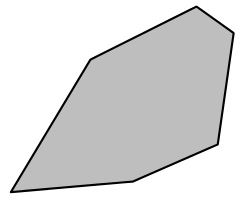
\includegraphics[width=0.33\textwidth]{gml.png}
    \caption{Пример кодирования многоугольника при помощи GML-разметки}
\end{figure}
\begin{lstlisting}[tabsize=2,breaklines,frame=single]{language=XML}
<gml:Polygon gml:id="p3" srsName="urn:ogc:def:crs:EPSG:6.6:4326">
	<gml:exterior>
		<gml:LinearRing>
			<gml:coordinates>5,5 28,7 44,14 47,35 40,40 20,30 5,5</gml:coordinates>
		</gml:LinearRing>
	</gml:exterior>
</gml:Polygon>
\end{lstlisting}

Open Geospatial Consortium (OGC) — международная некоммерческая организация, ведущая деятельность по разработке стандартов в сфере геопространственных данных и сервисов, созданная в 1994 году. В настоящее время координирует деятельность более 500 \cite{noauthor_open_nodate} правительственных, коммерческих, некоммерческих и научно-исследовательских организаций с целью разработки и внедрения консенсусных решений в области открытых стандартов для геопространственных данных, обработки данных геоинформационных систем и совместного использования данных. Большинство стандартов OGC основано на принципах, изложенных в базовой модели данных для представления географических характеристик под названием Abstract Specification. На основе базовой модели участники консорциума разработали и продолжают разрабатывать большое число спецификаций или стандартов для обслуживания конкретных потребностей организаций-участников в области геопространственных технологий и сервисов, включая ГИС.

Проект OpenGIS был инициирован до учреждения OGS, и впоследствии стал торговым знаком для ряда спецификаций, разрабатываемых и поддерживаемых в рамках этого консорциума. Стандарт GML определяет спецификацию географического языка разметки на основе синтаксиса XML. Этот язык позволяет кодировать географическую информацию, которая включает, в частности, геометрические характеристики объектов, в форме XML-документов. Такие документы могут использоваться для обмена геоданными между различными приложениями, обеспечивая их унификацию; для хранения геоданных и доступа к ним, в том числе и в среде глобальной сети; для публикации их на веб-сайтах. Разработка начальной версии языка GML (GML 1.0) была завершена весной 2000 года. Действующая в настоящее время версия этого стандарта - GML 3.3. Версия GML 3.1.0 была представлена консорциумом OGC в ISO в 1994 г. для создания на ее основе официального международного стандарта, где в настоящее время  эта спецификация проходит принятую в ISO процедуру стандартизации \cite{noauthor_iso_nodate}.

\begin{figure}[h]
    \centering
    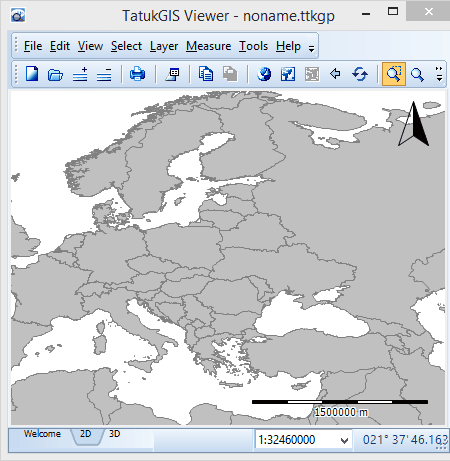
\includegraphics{tatuk.png}
    \caption{Интерфейс программы TatukGIS Viewer}
\end{figure}

Для работы с данными, закодированными в GML и сходных стандартах, компанией TatukGIS была разработана соответствующая линейка приложений. В частности, для визуализации данных в данной работе использовался TatukGIS Viewer.

\subsection{Существующие решения}
\label{}

Большинство алгоритмов упрощения топологии ГИС-файлов предназначаются для количественных преобразований (уменьшение размера файла), а не качественных. Однако, подобные задачи возникают в теории дифференциальных уравнений в частных производных и теории функций комплексной переменной --- в частности, при доказательстве интегральной теоремы Коши для многосвязной области \cite{__nodate}; а также в теории дифференциальных уравнений в частных производных --- например, при решении уравнения Лапласа в многосвязной области \cite{crowdy_transform_2015}.

\begin{figure}[h]
    \centering
    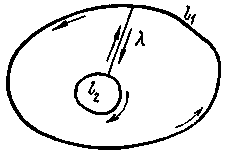
\includegraphics[width=0.4\textwidth]{koshi.png}
    \caption{Интегральная теорема Коши для многосвязной области}
\end{figure}

Задача \ref{task2}, а, точнее, ее предельный случай при $N=3$ (задача о триангуляции многоугольника \cite{de_berg_chapter_2000}), широко известна в области трехмерной графики, поскольку в ней треугольник является фундаментальной единицей для составления более сложных объектов. Однако, прямое использование алгоритма триангуляции для решения задачи \ref{task2} очень неэффективно.

\begin{figure}[h]
    \centering
    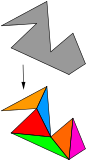
\includegraphics[width=0.2\textwidth]{triangulation.png}
    \caption{Задача о триангуляции многоугольника}
\end{figure}

\subsection{Теоретические сведения}
\label{}

\subsubsection{Топология}
\label{}

\textbf{Топология} --- раздел математики, занимающийся изучением свойств фигур (или пространств), которые сохраняются при непрерывных деформациях, таких, например, как растяжение, сжатие или изгибание. Непрерывная деформация – это деформация фигуры, при которой не происходит разрывов (т.е. нарушения целостности фигуры) или склеиваний (т.е. отождествления ее точек). Такие геометрические свойства связаны с положением, а не с формой или величиной фигуры.

Одной из характеристик фигур, инвариантных относительно непрерывных деформаций, является порядок связности. В \ref{task1} использовалось понятие односвязности. В простейшем двумерном случае односвязная фигура --- такая, в которой любой замкнутый путь можно непрерывно стянуть в точку. Проще говоря, это фигура, в которой отсутствуют <<дыры>>. Двусвязная область имеет одну дыру, трехсвязная – две, и т.д. При этом форма областей и дыр не имеет значения \cite{__2012}.

\begin{figure}[h]
    \centering
    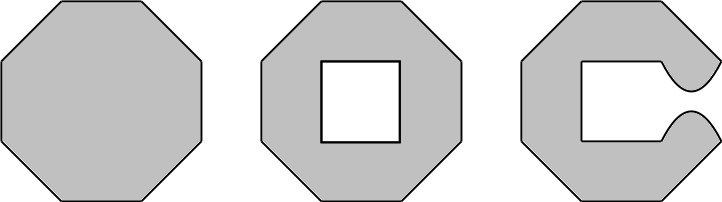
\includegraphics[width=1\textwidth]{topology.png}
    \caption{Слева направо: односвязная область, двусвязная область, преобразование двусвязной области в односвязную}
\end{figure}

Поскольку поставленная задача состоит в изменении порядка связности, конкретно --- в его уменьшении, она не может быть решена при помощи непрерывных деформаций. Требуется внести в многосвязные области разрезы при минимальном изменении их существенных характеристик. Эта цель достигается при помощи вырожденных туннелей: отрезок, по которому производится разрез, дважды вносится в границу результирующей области, благодаря чему площадь области не изменяется.

\begin{figure}[ht]
    \centering
    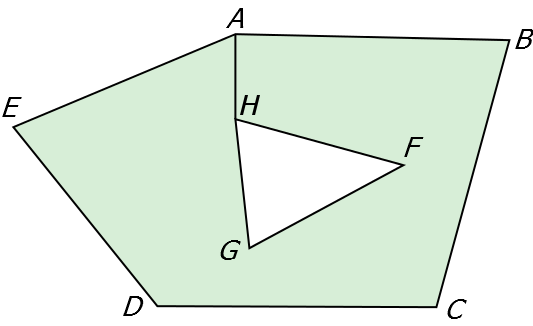
\includegraphics[width=0.7\textwidth]{reduce.png}
    \caption{Упрощение топологии полигональной области: $ABCDE \setminus FGH = ABCDEAHGFHA$}
    \label{fig:polysimp}
\end{figure}

\subsubsection{Теория графов}
\label{}

Для решения задачи \ref{task1} будет использован \textit{алгоритм Прима} из теории графов.

Граф – это совокупность двух множеств: множества точек, которые называются вершинами, и множества ребер А. Ребра --- это неупорядоченные (для неориентированного графа) или упорядоченные (для ориентированного) пары элементов из множества вершин, которые называются концами ребра. Если каждому ребру сопоставляется некоторое число (вес), то граф называется взвешенным. 

Дерево --- это граф, не имеющий циклов, т.е. замкнутых путей. Остов графа --- это его подграф, содержащий все вершины исходного, но являющийся деревом. Минимальный остов взвешенного графа --- это остовное дерево, имеющее наименьший суммарный вес ребер \cite{__2010}.

Алгоритм Прима используется для поиска в неориентированном взвешенном графе минимального остовного дерева. В нем искомый минимальный остов строится постепенно, путем добавлением в него ребер по одному. Изначально остов полагается состоящим из единственной вершины, взятой произвольно. Затем выбирается ребро минимального веса, исходящее из этой вершины, и добавляется в минимальный остов. Далее на каждом шаге ищется минимальное по весу ребро, один конец которого — уже взятая вершина, а другой — ещё не взятая, и это ребро добавляется в остов (если таких рёбер несколько, можно взять любое). Этот процесс повторяется до тех пор, пока остов не будет содержать все вершины \cite{prim_shortest_1957}. Без дополнительных оптимизаций алгоритм Прима работает за квадратичное время.

Альтернативой алгоритма Прима является алгоритм Краскала. В нем текущее множество ребер вначале устанавливается пустым. Затем, пока это возможно, проводится следующая операция: из всех рёбер, добавление которых к уже имеющемуся множеству не вызовет появление в нём цикла, выбирается ребро минимального веса и добавляется к уже имеющемуся множеству. Когда таких рёбер больше нет, алгоритм завершён. Подграф данного графа, содержащий все его вершины и найденное множество рёбер, является его остовным деревом минимального веса \cite{kruskal_shortest_1956}.

Можно показать, что в пределе время выполнения алгоритма Прима пропорционально количеству вершин \cite{prim_shortest_1957}, а алгоритма Краскала --- количеству ребер \cite{kruskal_shortest_1956}. Поскольку в данной работе требуется искать минимальный остов в графах, близких к полным, оптимально будет использование алгоритма Прима. Кроме того, он проще в реализации.
\section{Общая методология}
\label{method}

\subsection{Требование 1}
\label{task1}

Формулировка требования: <<Отсутствуют вложенные области, т.е. все области односвязны>>.

Многосвязная область состоит из внешней границы и произвольного числа внутренних границ, заданных многоугольниками. Задача снижения порядка связности области сводится к выбору соединений точек различных границ таким образом, чтобы все они оказались связаны. В простейшем случае с одной внутренней границей подойдет любой отрезок, один из концов которого принадлежит множеству вершин внешней границы, а другой --- внутренней, и который не имеет с границами других общих точек. В случае трехсвязной области (с двумя внутренними границами) можно также соединить внутренние границы, а затем одну из них --- со внешней.

Чтобы найти требуемые соединения, преобразуем объектную модель карты следующим образом. Поставим в соответствие каждому многоугольнику, включая внешнюю границу, вершину графа и сделаем полученный граф полным. В полученной графовой модели ребра соответствуют соединениям между многоугольниками. В качестве весов присвоим им длины кратчайших соединений между соответствующими многоугольниками. Далее, нужно исключить из модели недопустимые соединения --- такие, которые имеют более двух общих точек с многоугольниками. Для этого будем проверять соединение на пересечение со всеми сторонами многоугольников в рассматриваемой области. Наконец, к полученному графу применим алгоритм Прима \cite{prim_shortest_1957} для выделения минимального остовного дерева.

\begin{figure}[h]
    \centering
    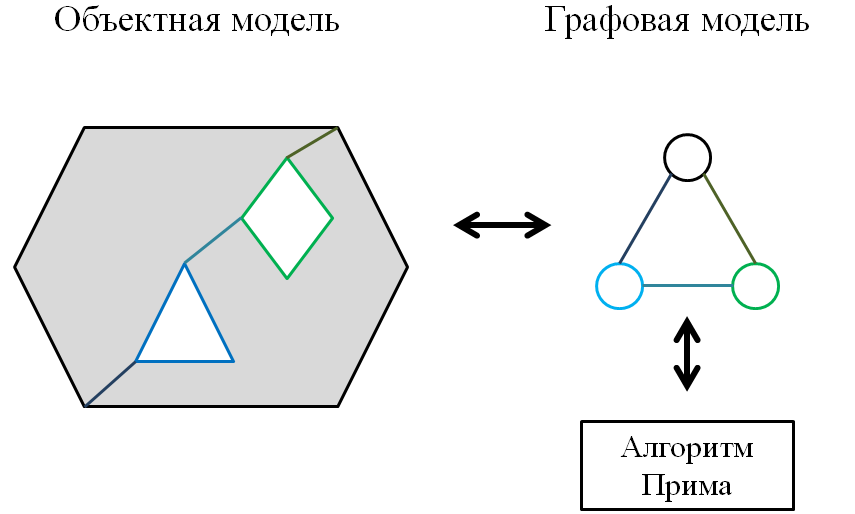
\includegraphics[width=1\textwidth]{Prim.png}
    \caption{Использование алгоритма Прима для удовлетворения требованию 1}
    \label{fig:prim}
\end{figure}

Восстановление объектной модели из графовой происходит следующим образом. На внешней границе произвольно выбирается начальная точка. Если с ней не связано ни одно из соединений в графовой модели, происходит переход к следующей вершине в том же многоугольнике; в противном случае эта вершина сохраняется в памяти, а следующей выбирается точка, находящаяся на другом конце найденного соединения, для которой та же процедура повторяется рекурсивно. Когда процесс возвращается в исходную точку, он возвращается по тому же соединению к предыдущему многоугольнику. Алгоритм завершает работу, когда возвращаться становится некуда. В результате вместо многосвязной области получается односвязная, в которой соединения становятся вырожденными туннелями.

\subsection{Требование 2}
\label{task2}

Формулировка требования: <<Число точек, задающих границу каждой области, не превышает заданной константы N>>. На данном этапе все области уже односвязны.

\begin{figure}[h]
    \centering
    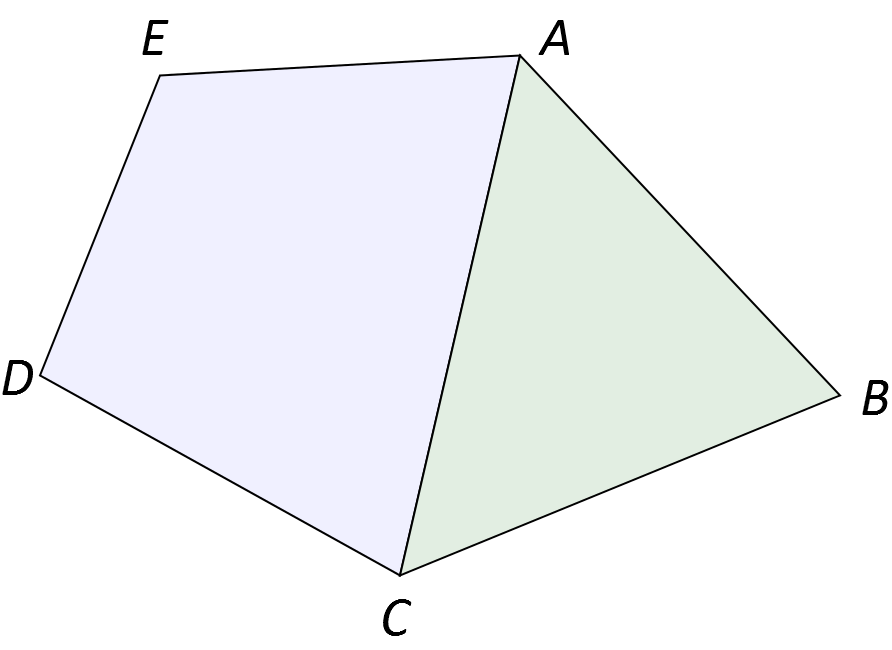
\includegraphics[width=0.6\textwidth]{split.png}
    \caption{Пример разбиения пятиугольника при максимальном количестве вершин N=4: $ABCDE = ABC \cup ACDE$}
\end{figure}

Рассмотрим вначале область, задаваемую выпуклым многоугольником с более чем N вершинами. Из определения выпуклости очевидно, что ее можно разделить в произвольном отношении, т.к. любая линия, соединяющая несмежные точки, будет лежать внутри области. С учетом требования 3 следует выбрать кратчайшую линию, разделяющую многоугольник таким образом, чтобы в одной из полученных частей было ровно N вершин. Если во второй части их больше N, повторяем ту же процедуру для нее рекурсивно.

Отметим, что при разбиении выпуклого многоугольника получаются также выпуклые многоугольники, поскольку все вершины полученных многоугольников лежат по одну и ту же сторону от новой грани.

Рассмотрим теперь невыпуклые многоугольники. Согласно \cite{de_berg_chapter_2000}, любой многоугольник можно разбить на смежные треугольники. Очевидно, эти треугольники можно объединять по смежным сторонам, получая таким образом разбивку на части с произвольным количеством вершин. Следовательно, существует и такая разбивка, при которой одна из частей имеет ровно N вершин. Значит, описанный алгоритм можно распространить и на невыпуклые области.

\subsection{Требование 3}
\label{}

Формулировка требования: <<Количество добавочных соединений и их длины минимальны>>. В процессе разработки к этому условию было добавлено важное уточнение: если минимизация обоих параметров одновременно невозможна или невыполнима за полиномиальное время, приоритет имеет количество соединений.

Докажем, что после выполнения описанных выше шагов алгоритма это условие уже выполнено.

Вначале рассмотрим добавочные соединения, образовавшиеся в процессе упрощения топологии. Вспомним, что эти соединения представляют собой остовное дерево в графе всевозможных соединений, причем за вес ребра в этом графе принимается длина соединения.

По свойству дерева \cite{__2010}, количество его ребер фиксировано: $B-P=1$, где $B$ — число вершин, $P$ — число рёбер графа. Следовательно, удаление любого из оставшихся соединений приведет к тому, что объект карты перестанет быть односвязным. Значит, условие минимальности количества дополнительных соединений выполняется.

Для выбора минимальных соединений из графа всех возможных соединений использовался алгоритм Прима. Из его корректности \cite{prim_shortest_1957} следует, что выбранное остовное дерево графа является минимальным. Значит, условие минимальности длин дополнительных соединений выполняется. Таким образом, требование 3 удовлетворено.

Теперь рассмотрим добавочные соединения, образовавшиеся в процессе уменьшения числа вершин.

Пусть дан многоугольник с $V$ вершинами. Тогда описанный выше алгоритм разобьет его на $M$ частей, причем $(M-1)*N < V+2*M \leq M*N$ (слагаемое $2M$ добавляется за счет того, что вершины, через которые проводится разделяющая линия, дублируются в результирующих многоугольниках). Очевидно, что при уменьшении $M$ на единицу количество вершин как минимум одного полученного после разбиения многоугольника будет превышать $M$; следовательно, условие минимальности количества дополнительных соединений выполняется.

Одновременная минимизация добавочных соединений и их длины теоретически возможна, но также требует полиномиального времени выполнения. С учетом примечания к требованию 3, решено было ограничиться результатами разработанного алгоритма, который дает оптимальное или близкое к оптимальному решение в большинстве практических случаев.

\subsection{Требование 4}
\label{}

Выполнение требования 4 очевидно, т.к. ни один из описанных выше алгоритмов не создавал новых вершин.

\subsection{Проверка допустимости соединений}
\label{}

Выше упоминалась проверка проводимых линий на допустимость, т.е. на пересечение с уже существующими линиями. Эта процедура является важной частью алгоритма, т.к. даже одно пропущенное пересечение делает непригодным весь выходной файл.

\begin{figure}[!htb]
    \centering
    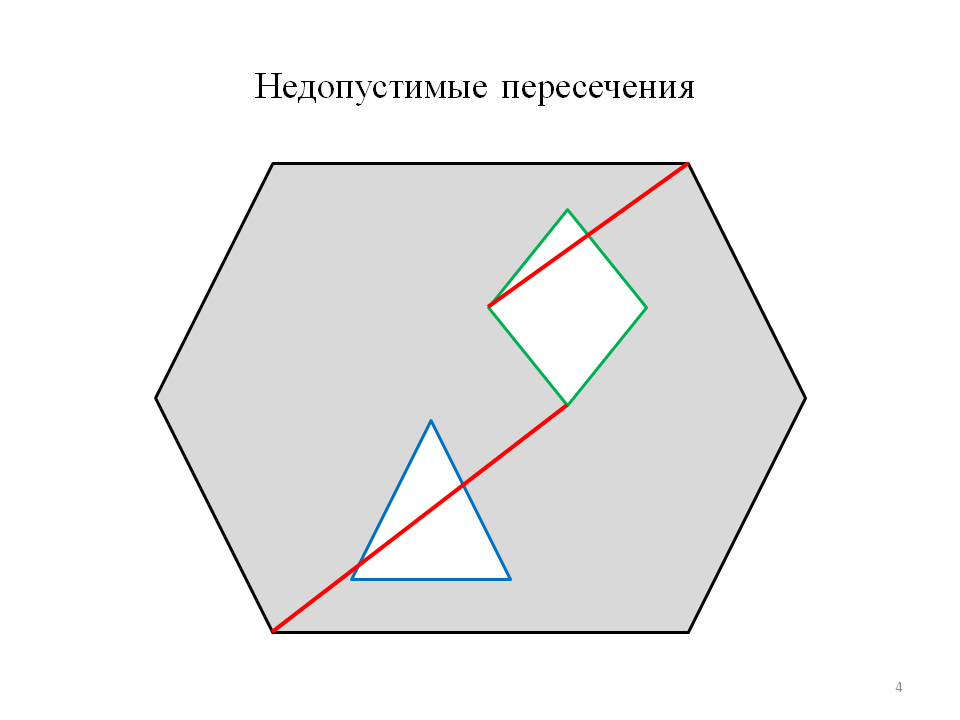
\includegraphics[width=1\textwidth]{errors.png}
    \caption{Примеры недопустимых соединений (выделены красным)}
    \label{fig:errors}
\end{figure}

Единственный способ убедиться в отсутствии недопустимых соединений --- проверять каждое проводимое соединение на пересечение с каждой из линий, составляющих границы области. Для этого используется алгоритм, описанный в \cite{noauthor_introduction_2009}.

Этот алгоритм основывается на понятии ориентации. Ориентация упорядоченного списка из трех точек в зависимости от их взаимного расположения может принимать три значения:

\begin{itemize}[noitemsep]
\item по часовой
\item против часовой
\item лежат на одной прямой
\end{itemize}

Два отрезка, $(p1,q1)$ и $(p2,q2)$, пересекаются тогда и только тогда, когда верно одно из условий (см. рис. \ref{fig:segments1}):

\begin{itemize}[noitemsep]
\item $(p1, q1, p2)$ и $(p1, q1, q2)$ имеют разную ориентацию
\item $(p2, q2, p1)$ и $(p2, q2, q1)$ имеют разную ориентацию
\end{itemize}

\begin{figure}[!h]
    \centering
    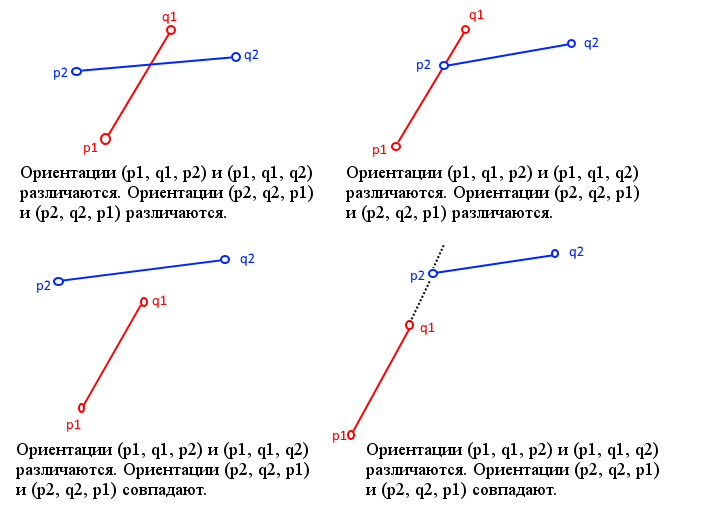
\includegraphics[width=1\textwidth]{linesegments.png}
    \caption{Возможные ориентации отрезков в общем случае}
    \label{fig:segments1}
\end{figure}

Отдельно следует рассмотреть случай коллинеарных отрезков. Они пересекаются, если одновременно выполняются условия (см. рис. \ref{fig:segments2}):

\begin{itemize}[noitemsep]
\item $(p1, q1, p2)$, $(p1, q1, q2)$, $(p2, q2, p1)$, и $(p2, q2, q1)$ лежат на одной прямой
\item проекции на ось $x$ отрезков $(p1, q1)$ и $(p2, q2)$ пересекаются
\item проекции на ось $y$ отрезков $(p1, q1)$ и $(p2, q2)$ пересекаются
\end{itemize}

\begin{figure}[!h]
    \centering
    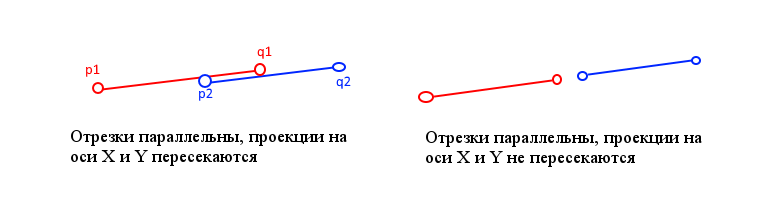
\includegraphics[width=1\textwidth]{linesegments2.png}
    \caption{Возможные ориентации коллинеарных отрезков}
    \label{fig:segments2}
\end{figure}

Докажем теперь, что проверять сами соединения на пересечения друг с другом не требуется. Для \ref{task2} утверждение очевидно: описанный алгоритм на каждом шаге исследует лишь одно соединение.

В \ref{task1} после построения полного графа допустимых соединений возникают пересечения. Однако, после выполнения алгоритма Прима они исчезнут. Почему? Предположим противное: в минимальном остовном дереве имеются ребра, соответствующие пересекающимся соединениям. Поменяем концы этих соединений таким образом, чтобы не нарушить связность графа (это всегда можно сделать, т.к. количество ребер графа не изменяется). Окажется, что длина каждого из полученных соединений меньше, чем у первоначальных. Но это противоречит корректности алгоритма Прима. Тем самым, утверждение доказано.
\section{Реализация алгоритма}
\label{}

Требования, предъявленные к разрабатываемому исполняемому файлу:
\begin{enumerate}
\item Время исполнения для предоставленных файлов-примеров имеет порядок секунд или минут. Возможность работы в реальном времени не требуется.
\item Целевая платформа --- Microsoft Windows. Доступны инструменты .NET Framework.
\item Графический интерфейс не требуется, т.к. взаимодействие программы с пользователем минимально.
\end{enumerate}

Кроме того, для работы с большими массивами структур данных требуются инструменты высокого уровня. Исходя из этих требований, для реализации алгоритма был выбран язык C\#: он полностью поддерживается платформой .NET Framework и обладает высокоуровневым инструментарием LINQ. В качестве среды разработки выбрана Microsoft Visual Studio 2013.

\subsection{Интерфейс}
\label{}

Выбор файлов для обработки реализован при помощи вызова системного диалога Windows через класс OpenFileDialog .NET Framework. После этого вывод отладочной информации осуществляется через текстовый интерфейс.

\begin{figure}[!htb]
    \centering
    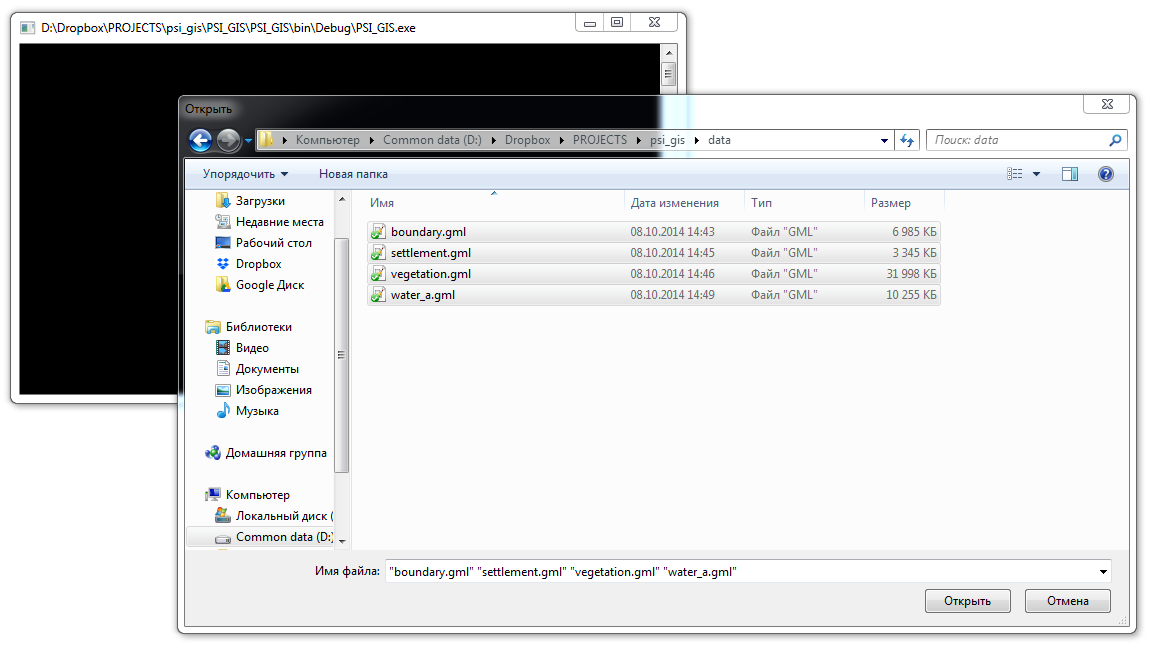
\includegraphics[width=1\textwidth]{dialog.png}
    \caption{Интерфейс ввода данных}
    \label{fig:dialog}
\end{figure}

\subsection{Объектная модель}
\label{}

\begin{center}
\begin{tikzpicture}
\umlclass[x=4,y=-13]{Vertex}{
  X, Y : double
}{
 distance(v : Vertex) : double
}
\umlclass[x=-5,y=-13]{Line}{
  a, b : Vertex
}{
 intersects(l : Line) : bool \\
 length() : double
}
\umlclass[x=-0.5,y=-7]{Poly}{
  vert : Vertex[]
}{
 Poly(XML : string) \\
 toXML() : XElement \\
 clearPath(v0, v1 : int) : bool \\
 reduce(poly : Poly) : Poly
}
\umlclass[x=4]{OuterPoly}{
  IP : Poly[] \\
  cutsGraph : int[,]
}{
 lineAllowed(line : Line) : bool \\
 shortestN2(p0, p1 : int) : int[2] \\
 buildPath(p0, p1 : int) : void \\
 Prim() : void \\
 unite() : void
}
\umlclass[x=-5]{FeatureMember}{
  pols : list<Poly> \\
  context : XElement \\
}{
 FeatureMember(node : XElement) \\
 toXML() : XElement
}
\umlunicompo[]{Line}{Vertex}
\umlunicompo[geometry=-|, anchor1=-20]{Poly}{Vertex}
\umlunicompo[geometry=|-, stereo=list]{FeatureMember}{Poly}
\umlunicompo[geometry=|-, stereo=array, anchor2=20]{OuterPoly}{Poly}
\end{tikzpicture}
\end{center}

\begin{itemize}
\item \textbf{Vertex}: базовый класс, представляет точку на плоскости.
\item \textbf{Line}: представляет отрезок. Состоит из двух объектов Vertex. Содержит методы для измерения длины и проверки пересечения с другим отрезком.
\item \textbf{Poly}: Общее представление многоугольника. Состоит из объектов Vertex. Реализует методы прямого и обратного преобразования в GML-элемент (Poly, toXML). Метод ClearPath проверяет, можно ли соединить две вершины многоугольника, не пересекая при этом его сторон. Метод reduce реализует алгоритм, описанный в \ref{task2}.
\item \textbf{OuterPoly}: Представляет многосвязную область. Состоит из внешней границы, представляемой объектом Poly, и массива многоугольников (IP), представляющих <<дыры>>. Метод lineAllowed проверяет, можно ли провести внутри области отрезок, не пересекающий сторон ни одного из составляющих ее многоугольников. Метод shortestN2 определяет кратчайший отрезок, соединяющий два многоугольника внутри области. Метод unite реализует алгоритм, описанный в \ref{task1} при помощи методов buildPath для построения полного графа соединений и Prim для алгоритма Прима.
\item \textbf{FeatureMember}: хранит метаданные областей, не имеющие отношения к их геометрии. Реализует ввод и вывод в GML.
\end{itemize}

\subsection{Пример работы}
\label{}

См. рис. \ref{fig:nocuts} и \ref{fig:result}.

\begin{figure}[!htb]
    \centering
    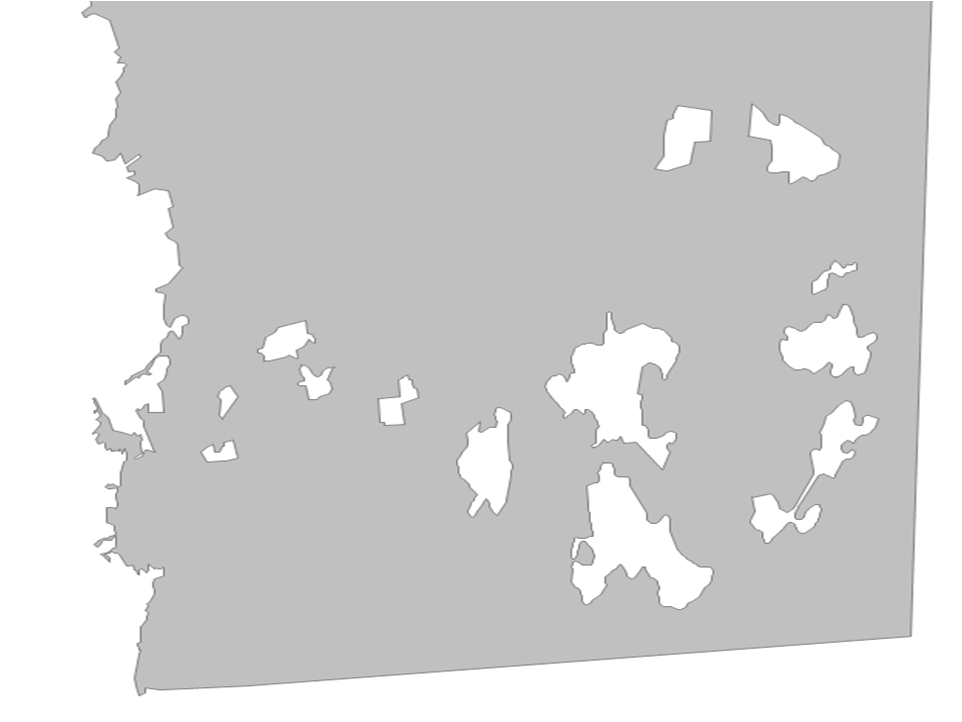
\includegraphics[width=1\textwidth]{nocuts.png}
    \caption{Визуализация фрагмента входного файла}
    \label{fig:nocuts}
\end{figure}

\begin{figure}[!htb]
    \centering
    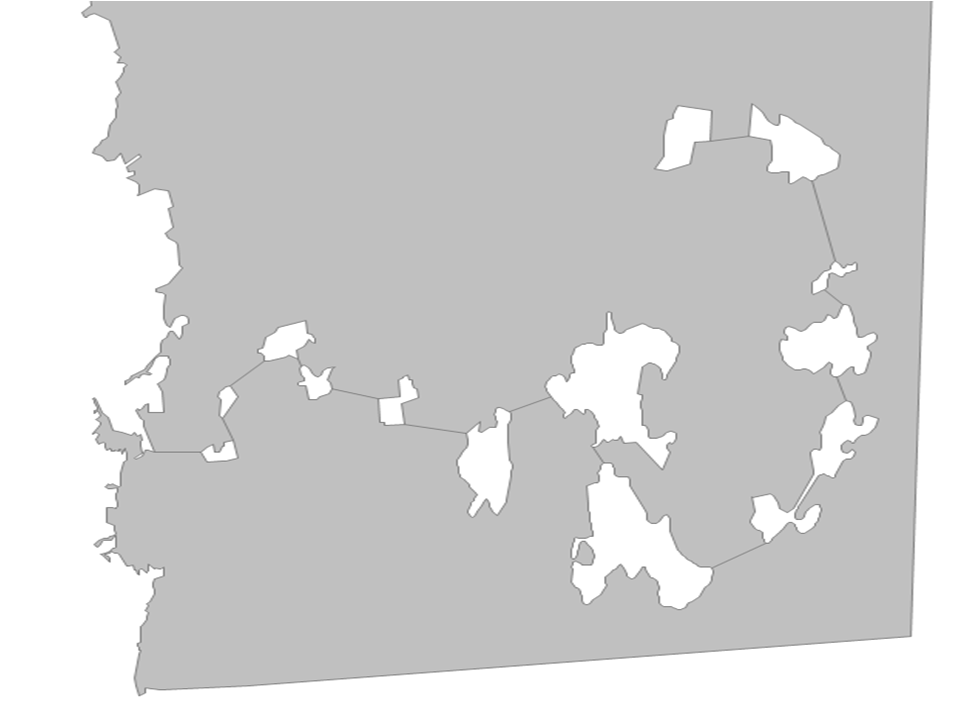
\includegraphics[width=1\textwidth]{result.png}
    \caption{Результат преобразования фрагмента файла}
    \label{fig:result}
\end{figure}
\section{Заключение}
\label{}

В рамках данной работы была разработана программа для программно-технического комплекса (ПТК) Автоматизированной системы диспетчерского управления (АСДУ) электрическими сетями PSIcontrol по оптимизации геоинформационных полигоннальных (замкнутых) структур данных на основе математической обработки входных XML-файлов по следующим критериям:

\begin{enumerate}
\item оптимальное перекрытие островных структур на случай их наличия в глобальной структуре без взаимных пересечений с использованием вырожденных туннелей;
\item оптимальное разрезание полигонов, содержащих значительное количество точек, на более мелкие полигоны, количество точек которых не превышает N.
\end{enumerate}

Результаты работы позволили снять ряд существенных ограничений по внедрению ГИС-системы ПТК АСДУ PSIcontrol, что позволило существенно (на два-три порядка) сократить время предварительной обработки геоинформационных подложек для ПТК.

Результаты работы внедрены в практическую деятельность Департамента энергетики ООО «ПСИ» и используются во всех текущих проектах компании по созданию и модернизации АСДУ на предприятиях российской электроэнергетики.

\printbibliography[heading=bibintoc]

\end{document}
